\documentclass{ROS}
\usepackage{paracol}
\usepackage[nosumlimits]{amsmath}
\usepackage{amsfonts}
\begin{document}


% \maketitle{Übungsnummer}{Abgabedatum}{removed}{Gruppennummer}
%           {TeilnehmerIn 1}{TeilnehmerIn 2}{TeilnehmerIn 3}

\maketitle{1}{16.11.2020}{}{7}
          {Shiyao~Zhang}{}

\section*{Exercise 1.} 
\subsubsection*{1.3 Steering}
A table describing what each of these buttons do.\\
\\
\begin{tabular}{|c|c|}
\hline
u&Circle ahead to the left\\
\hline
i&Steer straight ahead\\
\hline
o&Circle ahead to the right\\
\hline
j&Rotation by counter clockwise\\
\hline
k&Stop steering\\
\hline
l&Rotation by clockwise\\
\hline
m&Circle backwards to the left\\
\hline
,&Steer straight back\\
\hline
.&Circle backwards to the right\\
\hline
q&increase speed\\
\hline
z&decrease speed\\
\hline
\end{tabular}
\\
\subsubsection*{1.4 Pictures!}
Here is a picture that shows the working simulator where I drive the robot close to the top-right pillar of the arena.\\
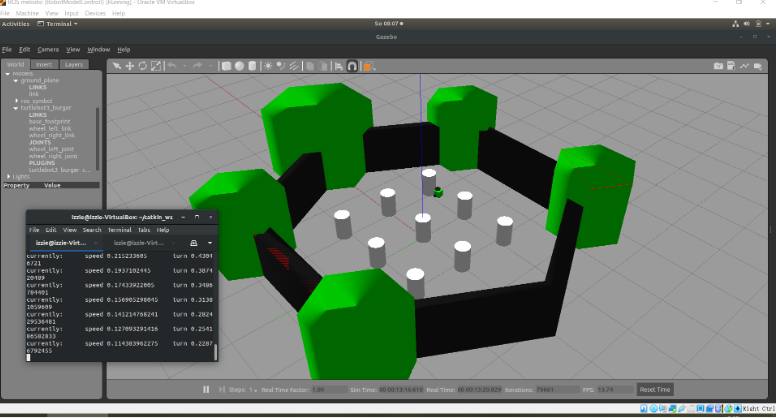
\includegraphics{Screenshot1.png}
\\
\section*{Exercise 2.}
\subsubsection*{What is the difference between rosrun and roslaunch?}
rosrun can only execute a single node from a single package while roslauch could launch two or more nodes from multiple packages at a time. Meanwhile roslaunch does put each node into its own process and pipe the output of that node to a log file. Whereas rosrun generates no log file. Rosrun like a shortcut execute a node in the terminal.In my opinion roslaunch could be tracked but rosrun not.\\
\\
\subsubsection*{What dose the command $"rosmsg show std_msgs/String"$ do?}
This command displays the fields in a ROS message type. Here the type is string. I may omit the package name of the type String, in which case rosmsg will search for matching type String in all packages.\\ 
\\
\subsubsection*{How can you make sure that a node is subscribing to a topic?}
Using rostopic echo. It shows the data published and subscribed on a topic.\\
rostopic echo [topic]\\
Using rostopic list. It returns a list of all topics currently subscribed to and pulished. When we press the options -s after print the command, it could return only subsribers.\\
\\
\section*{Exercise 3.}
\subsubsection*{Batteries lose capatity over time. What do you need to do to assure a long lifetime of a battery?}
First of all, everyone should use the battery with safty instructions.Safe battery usage abd storing batteries in a correct way would assure a long lifetime of a battery.\\
For example about safe battery usage:\\
1.Don't let the battery get empty.\\
2.Assure good operation temperature. When the battery's temperature goes up, it should stop to be using until the temperature is close to normal.\\
3.Fix the battery in a correct position and couldn't be moved anywhere, when the battery is used.\\
4.Do not apply physical stress on the battery like huge pressure on the surface.\\
5.Balance all cells from time to time so they discharge equally during use. \\
\\
For example about safe storing batteries:\\
1.Charge to 70 percent.\\
2.Use the storing program of the charger.\\
3.Check regularly, at least every 3 months.\\
4.Store in special fire-proof boxes with integrated estinguishing agent. Meanwhile assure the right temperature. Inside the batteries chemical matterials would be reacted in fire or in a high temperature.\\

\subsubsection*{What can you do to prevent your battery from exploding?}
1.Store the batteries away from fire and high temperature.\\
2.Avoid the overuse of batteries. Because overuse will lead to a higher temperature inside the batteries.\\
3.Do not use the batteries during the charging.\\
4.Stop using the batteries as soon as possible when it has been damaged or some index was unusual after the check.\\
\\

\section*{Exercise 4 Moin, ROS!}
\subsubsection*{4.1 Some Code\\Explain what happens when we call the function "schnacker" in the following code:}
\begin{lstlisting}[firstnumber=1]
#!/user/bin/env python # The script is executed as a Python script.
import rospy # Import rospy if we need to write a ROS Node.
from std_msgs.msg import String # After that we could reuse the std_msgs/String message type for publishing.

def schnacker():# We define a method named schnakcer.
    x = rospy.Publisher('chatter', String, queue_size=8) # The node is publishing to the chatter topic using the message type String. The queue_size method limits the amount of queued messages.
    rospy.init_node('talker', anonymous=True) # Tells rospy the name "talker" of the node. After rospy has had this information, it can start comminicating with the ROS Master. And "anonymous=True" means that it was ensured that the node has a unique name by adding random numbers to the end of NAME.
    repetitons = rospy.Rate(20) # With the help of its method sleep(), it offers a way for looping as the desired rate.Every second the loop will be executed 20 times.
    while not rospy.is_shutdown(): # Check the method rospy.is_shutdown() and go through the loop. That can enssure if the program should exit.
          foo = "Moin ROS! The timestamp is: \%s" \% rospy.get_time() # The string named foo is a sentence following by a current time. It was executed by a method rospy.get_time()
          x.publish(foo) # That published a string to out chatter topic
          repetitions.sleep()# The method sleeps enough to manintain the desired rate through the loop

if __name__ = '__main__': # In the standard Python __main__ check, this will catch a rospy.ROSInterruptException exception, which can throw by rospy.sleep() and rospy.Rate.sleep()when the node is shutdown by pressing Ctrl-c.
    try:
         schnacker()
    except rospy.ROSInterruptException:
         pass
\end{lstlisting}

\subsubsection*{4.2 Better documentation}
\begin{lstlisting}[firstnumber=1]
#!/user/bin/env python 
import rospy 
from std_msgs.msg import String

def talker(): # I have change schnaker to takler. The funktion of this method is broadcasting a message like a talker.
    pub = rospy.Publisher('chatter', String, queue_size=8) # I have changed x to pub, pub is abbreviation of publishment. I think that is easier to understand.
    rospy.init_node('talker', anonymous=True)
    rate = rospy.Rate(20) # I have changed repetitions to rate. This name is short and represents the meaning of this methods.
    while not rospy.is_shutdown():
          hello_str = "Moin ROS! The timestamp is: \%s" \% rospy.get_time() # I have change foo to hello_str. That string refers to the function of string while foo is just a name.  
          pub.publish(hello_str)
          rate.sleep()

if __name__ = '__main__':
    try:
         talker()
    except rospy.ROSInterruptException:
         pass
\end{lstlisting}
In my oponion a good documentation could lead readers to think about and understand it. For example the origin name foo. When I first time looked at this variable, I must to think about the meaning even though I could also by reading the assignment of foo get the meaning. But hello\_str is so easier to read. Therefore a name of variable is not only a symbol but also a real name that could transmit information to the readers.\\
\section*{Feedback}
\subsubsection*{How much time did you spendon doing this sheet per person}
I hava spent 8 hours.
\subsubsection*{Was is too easy, easy, ok, hard, too hard?}
Nothing is too easy\\
Installation followed the video: easy\\
Understanding the command: ok\\
Compare some details like rosrun roslauch: hard\\
Using the ROS without video and python program: too hard\\
\subsubsection*{What additional resources(blogs, papers, books, tutorials, etc) did you use?} 
\url{https://www.theconstructsim.com/ros-5-mins-008-difference-rosrun-roslaunch/}
\url{http://wiki.ros.org/ROS/Tutorials/WritingPublisherSubscriber%28python%29}
\url{http://wiki.ros.org/ROS/Tutorials/UnderstandingTopics}
\subsubsection*{Any other issue?}





\end{document}